\documentclass{beamer}
\usetheme{metropolis}

\usepackage{tikz}
\usepackage{overpic}

\title[Graph Neural Networks]{Machine Learning on Graphs\\ 
                              {\small\textsc{PyTorch London Meetup}}}
\author[Dan Saattrup Nielsen]{Dan Saattrup Nielsen\\ 
                              Danish Business Authority}
\date{November 3, 2020}

\begin{document}

\begin{frame}
	\titlepage
\end{frame}


%===== What is a graph? =====

\begin{frame}{An overview of the talk}
  \begin{enumerate}
    \item<alert@2> What is a graph?
    \item Which machine learning tasks can we do on graphs?
      \begin{enumerate}
        \item Node classification
        \item Graph classification
        \item Link prediction
      \end{enumerate}
    \item A zoo of algorithms
      \begin{enumerate}
        \item Transductive classification: DeepWalk
        \item Inductive classification: Graph convolutions
      \end{enumerate}
    \item PyTorch implementation
    \item Application: Fraud detection
  \end{enumerate}
\end{frame}

\begin{frame}{What is a graph?}
  \begin{center}
    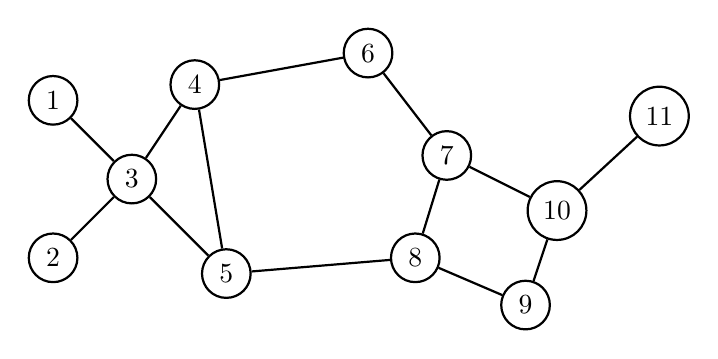
\begin{tikzpicture}
      \begin{scope}[every node/.style={circle,thick,draw}]
        \node (1) at (0,2) {1};
        \node (2) at (0,0) {2};
        \node (3) at (1,1) {3};
        \node (4) at (1.8,2.2) {4};
        \node (5) at (2.2,-0.2) {5};
        \node (6) at (4,2.6) {6};
        \node (7) at (5,1.3) {7};
        \node (8) at (4.6,0) {8};
        \node (9) at (6,-0.6) {9};
        \node (10) at (6.4,0.6) {10};
        \node (11) at (7.7,1.8) {11};
      \end{scope}
      \begin{scope}[every edge/.style={draw,thick}]
        \path (1) edge (3);
        \path (2) edge (3);
        \path (3) edge (4);
        \path (3) edge (5);
        \path (4) edge (5);
        \path (4) edge (6);
        \path (5) edge (8);
        \path (6) edge (7);
        \path (7) edge (8);
        \path (7) edge (10);
        \path (8) edge (9);
        \path (9) edge (10);
        \path (10) edge (11);
      \end{scope}
    \end{tikzpicture}
  \end{center}
\end{frame}


%===== Node classification =====

\begin{frame}{An overview of the talk}
  \begin{enumerate}
    \item What is a graph?
    \item<alert@1> Which machine learning tasks can we do on graphs?
      \begin{enumerate}
        \item<alert@2> Node classification
        \item Graph classification
        \item Link prediction
      \end{enumerate}
    \item A zoo of algorithms
      \begin{enumerate}
        \item Transductive classification: DeepWalk
        \item Inductive classification: Graph convolutions
      \end{enumerate}
    \item PyTorch implementation
    \item Application: Fraud detection
  \end{enumerate}
\end{frame}

\begin{frame}{Node classification}

  \invisible{Proximity classification:}
  \invisible{Structural classification:}

  \begin{center}
    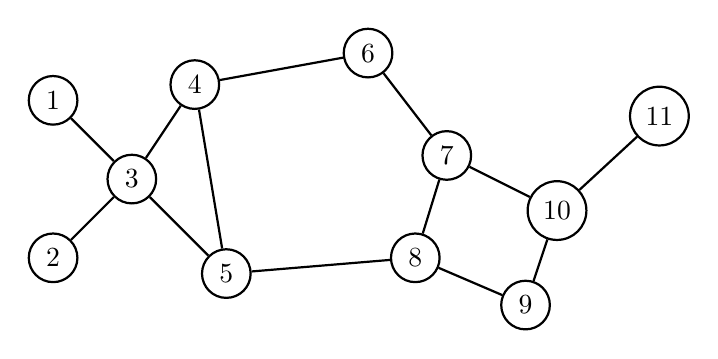
\begin{tikzpicture}
      \begin{scope}[every node/.style={circle,thick,draw}]
        \node (1) at (0,2) {1};
        \node (2) at (0,0) {2};
        \node (3) at (1,1) {3};
        \node (4) at (1.8,2.2) {4};
        \node (5) at (2.2,-0.2) {5};
        \node (6) at (4,2.6) {6};
        \node (7) at (5,1.3) {7};
        \node (8) at (4.6,0) {8};
        \node (9) at (6,-0.6) {9};
        \node (10) at (6.4,0.6) {10};
        \node (11) at (7.7,1.8) {11};
      \end{scope}
      \begin{scope}[every edge/.style={draw,thick}]
        \path (1) edge (3);
        \path (2) edge (3);
        \path (3) edge (4);
        \path (3) edge (5);
        \path (4) edge (5);
        \path (4) edge (6);
        \path (5) edge (8);
        \path (6) edge (7);
        \path (7) edge (8);
        \path (7) edge (10);
        \path (8) edge (9);
        \path (9) edge (10);
        \path (10) edge (11);
      \end{scope}
    \end{tikzpicture}
  \end{center}
\end{frame}

\begin{frame}{Node classification}

  Proximity classification:
  \invisible{Structural classification:}

  \begin{center}
    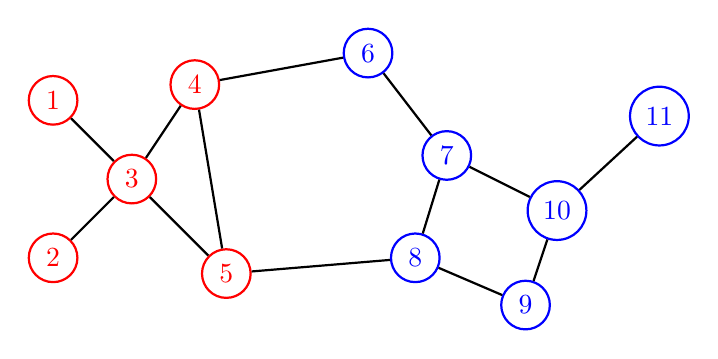
\begin{tikzpicture}
      \begin{scope}[every node/.style={circle,thick,draw}]
        \node[color=red] (1) at (0,2) {1};
        \node[color=red] (2) at (0,0) {2};
        \node[color=red] (3) at (1,1) {3};
        \node[color=red] (4) at (1.8,2.2) {4};
        \node[color=red] (5) at (2.2,-0.2) {5};
        \node[color=blue] (6) at (4,2.6) {6};
        \node[color=blue] (7) at (5,1.3) {7};
        \node[color=blue] (8) at (4.6,0) {8};
        \node[color=blue] (9) at (6,-0.6) {9};
        \node[color=blue] (10) at (6.4,0.6) {10};
        \node[color=blue] (11) at (7.7,1.8) {11};
      \end{scope}
      \begin{scope}[every edge/.style={draw,thick}]
        \path (1) edge (3);
        \path (2) edge (3);
        \path (3) edge (4);
        \path (3) edge (5);
        \path (4) edge (5);
        \path (4) edge (6);
        \path (5) edge (8);
        \path (6) edge (7);
        \path (7) edge (8);
        \path (7) edge (10);
        \path (8) edge (9);
        \path (9) edge (10);
        \path (10) edge (11);
      \end{scope}
    \end{tikzpicture}
  \end{center}
\end{frame}

\begin{frame}{Node classification}

  Structural classification:
  \invisible{Proximity classification:}

  \begin{center}
    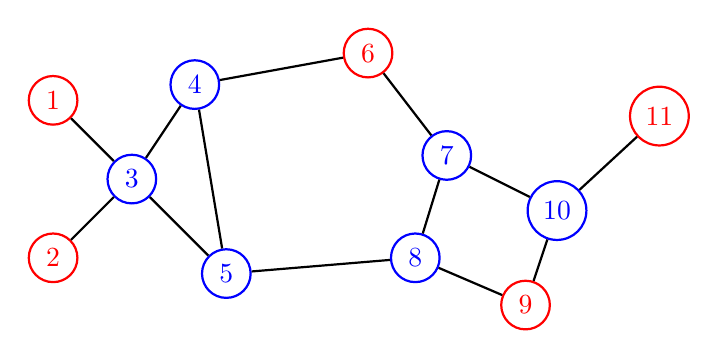
\begin{tikzpicture}
      \begin{scope}[every node/.style={circle,thick,draw}]
        \node[color=red] (1) at (0,2) {1};
        \node[color=red] (2) at (0,0) {2};
        \node[color=blue] (3) at (1,1) {3};
        \node[color=blue] (4) at (1.8,2.2) {4};
        \node[color=blue] (5) at (2.2,-0.2) {5};
        \node[color=red] (6) at (4,2.6) {6};
        \node[color=blue] (7) at (5,1.3) {7};
        \node[color=blue] (8) at (4.6,0) {8};
        \node[color=red] (9) at (6,-0.6) {9};
        \node[color=blue] (10) at (6.4,0.6) {10};
        \node[color=red] (11) at (7.7,1.8) {11};
      \end{scope}
      \begin{scope}[every edge/.style={draw,thick}]
        \path (1) edge (3);
        \path (2) edge (3);
        \path (3) edge (4);
        \path (3) edge (5);
        \path (4) edge (5);
        \path (4) edge (6);
        \path (5) edge (8);
        \path (6) edge (7);
        \path (7) edge (8);
        \path (7) edge (10);
        \path (8) edge (9);
        \path (9) edge (10);
        \path (10) edge (11);
      \end{scope}
    \end{tikzpicture}
  \end{center}
\end{frame}


%===== Graph classification =====

\begin{frame}{An overview of the talk}
  \begin{enumerate}
    \item What is a graph?
    \item Which machine learning tasks can we do on graphs?
      \begin{enumerate}
        \item Node classification
        \item<alert@1> Graph classification
        \item Link prediction
      \end{enumerate}
    \item A zoo of algorithms
      \begin{enumerate}
        \item Transductive classification: DeepWalk
        \item Inductive classification: Graph convolutions
      \end{enumerate}
    \item PyTorch implementation
    \item Application: Fraud detection
  \end{enumerate}
\end{frame}

\begin{frame}{Graph classification}
  \begin{center}
    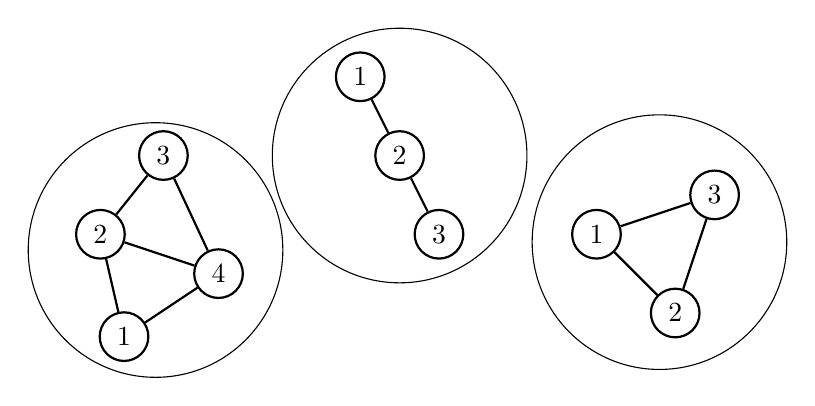
\begin{tikzpicture}

      % Nodes
      \begin{scope}[every node/.style={circle,thick,draw}]
        \node (01) at (0,0.2) {1};
        \node (02) at (-0.3,1.5) {2};
        \node (03) at (0.5,2.5) {3};
        \node (04) at (1.2,1) {4};

        \node (11) at (3,3.5) {1};
        \node (12) at (3.5,2.5) {2};
        \node (13) at (4,1.5) {3};

        \node (21) at (6,1.5) {1};
        \node (22) at (7,0.5) {2};
        \node (23) at (7.5,2) {3};
      \end{scope}

      % Edges
      \begin{scope}[every edge/.style={draw,thick}]
        \path (01) edge (02);
        \path (01) edge (04);
        \path (02) edge (03);
        \path (02) edge (04);
        \path (03) edge (04);

        \path (11) edge (12);
        \path (12) edge (13);

        \path (21) edge (22);
        \path (21) edge (23);
        \path (22) edge (23);
      \end{scope}

      % Circles
      \begin{scope}[every node/.style={minimum size=92pt,circle,draw}]
        \node at (0.4,1.3) {};
        \node at (3.5,2.5) {};
        \node at (6.8,1.4) {};
      \end{scope}

    \end{tikzpicture}
  \end{center}
\end{frame}

\begin{frame}{Graph classification}
  \begin{center}
    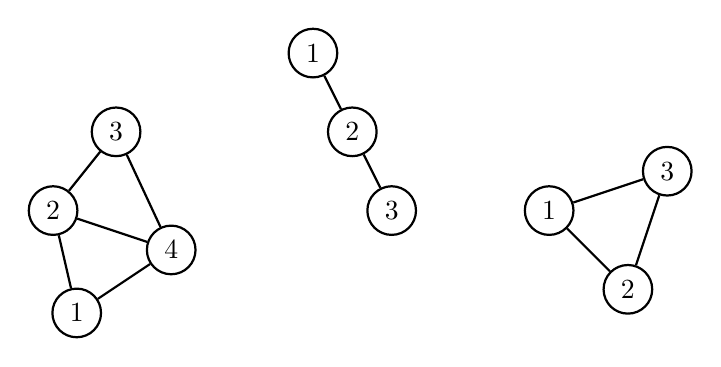
\begin{tikzpicture}

      % Nodes
      \begin{scope}[every node/.style={circle,thick,draw}]
        \node (01) at (0,0.2) {1};
        \node (02) at (-0.3,1.5) {2};
        \node (03) at (0.5,2.5) {3};
        \node (04) at (1.2,1) {4};

        \node (11) at (3,3.5) {1};
        \node (12) at (3.5,2.5) {2};
        \node (13) at (4,1.5) {3};

        \node (21) at (6,1.5) {1};
        \node (22) at (7,0.5) {2};
        \node (23) at (7.5,2) {3};
      \end{scope}

      % Edges
      \begin{scope}[every edge/.style={draw,thick}]
        \path (01) edge (02);
        \path (01) edge (04);
        \path (02) edge (03);
        \path (02) edge (04);
        \path (03) edge (04);

        \path (11) edge (12);
        \path (12) edge (13);

        \path (21) edge (22);
        \path (21) edge (23);
        \path (22) edge (23);
      \end{scope}

    \end{tikzpicture}
  \end{center}
\end{frame}

\begin{frame}{Graph classification}
  \begin{center}
    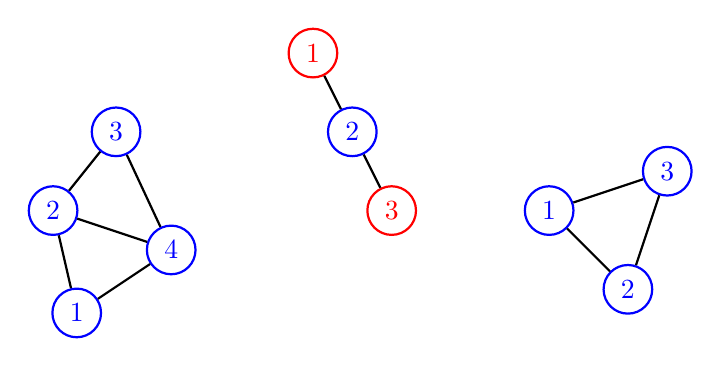
\begin{tikzpicture}

      % Nodes
      \begin{scope}[every node/.style={circle,thick,draw}]
        \node[color=blue] (01) at (0,0.2) {1};
        \node[color=blue] (02) at (-0.3,1.5) {2};
        \node[color=blue] (03) at (0.5,2.5) {3};
        \node[color=blue] (04) at (1.2,1) {4};

        \node[color=red] (11) at (3,3.5) {1};
        \node[color=blue] (12) at (3.5,2.5) {2};
        \node[color=red] (13) at (4,1.5) {3};

        \node[color=blue] (21) at (6,1.5) {1};
        \node[color=blue] (22) at (7,0.5) {2};
        \node[color=blue] (23) at (7.5,2) {3};
      \end{scope}

      % Edges
      \begin{scope}[every edge/.style={draw,thick}]
        \path (01) edge (02);
        \path (01) edge (04);
        \path (02) edge (03);
        \path (02) edge (04);
        \path (03) edge (04);

        \path (11) edge (12);
        \path (12) edge (13);

        \path (21) edge (22);
        \path (21) edge (23);
        \path (22) edge (23);
      \end{scope}

    \end{tikzpicture}
  \end{center}
\end{frame}

\begin{frame}{Graph classification}
  \begin{center}
    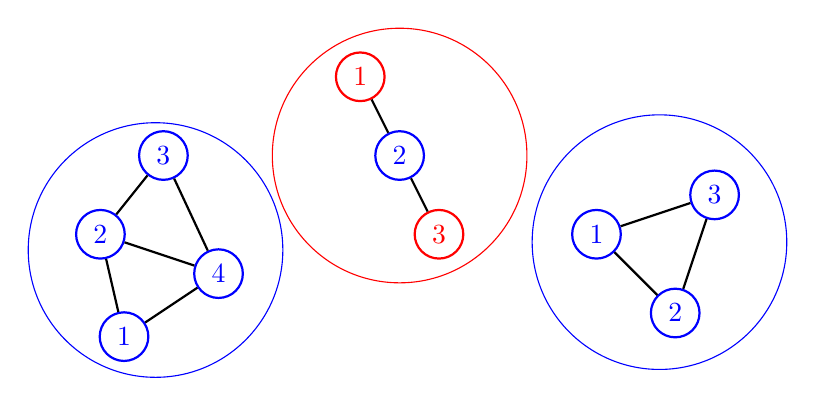
\begin{tikzpicture}

      % Nodes
      \begin{scope}[every node/.style={circle,thick,draw}]
        \node[color=blue] (01) at (0,0.2) {1};
        \node[color=blue] (02) at (-0.3,1.5) {2};
        \node[color=blue] (03) at (0.5,2.5) {3};
        \node[color=blue] (04) at (1.2,1) {4};

        \node[color=red] (11) at (3,3.5) {1};
        \node[color=blue] (12) at (3.5,2.5) {2};
        \node[color=red] (13) at (4,1.5) {3};

        \node[color=blue] (21) at (6,1.5) {1};
        \node[color=blue] (22) at (7,0.5) {2};
        \node[color=blue] (23) at (7.5,2) {3};
      \end{scope}

      % Edges
      \begin{scope}[every edge/.style={draw,thick}]
        \path (01) edge (02);
        \path (01) edge (04);
        \path (02) edge (03);
        \path (02) edge (04);
        \path (03) edge (04);

        \path (11) edge (12);
        \path (12) edge (13);

        \path (21) edge (22);
        \path (21) edge (23);
        \path (22) edge (23);
      \end{scope}

      % Circles
      \begin{scope}[every node/.style={minimum size=92pt,circle,draw}]
        \node[color=blue] at (0.4,1.3) {};
        \node[color=red] at (3.5,2.5) {};
        \node[color=blue] at (6.8,1.4) {};
      \end{scope}

    \end{tikzpicture}
  \end{center}
\end{frame}

%===== Link prediction =====

\begin{frame}{An overview of the talk}
  \begin{enumerate}
    \item What is a graph?
    \item Which machine learning tasks can we do on graphs?
      \begin{enumerate}
        \item Node classification
        \item Graph classification
        \item<alert@1> Link prediction
      \end{enumerate}
    \item A zoo of algorithms
      \begin{enumerate}
        \item Transductive classification: DeepWalk
        \item Inductive classification: Graph convolutions
      \end{enumerate}
    \item PyTorch implementation
    \item Application: Fraud detection
  \end{enumerate}
\end{frame}

\begin{frame}{Link prediction}
  \begin{center}
    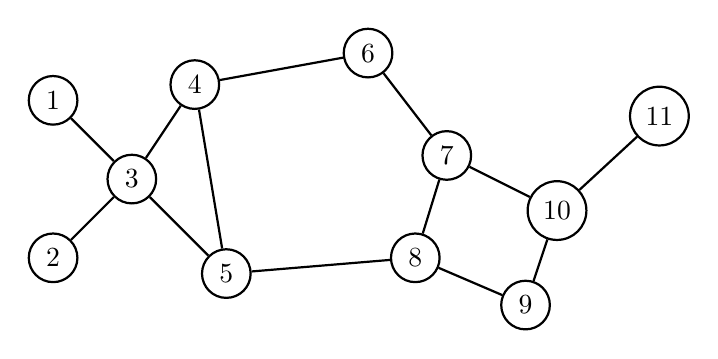
\begin{tikzpicture}
      \begin{scope}[every node/.style={circle,thick,draw}]
        \node (1) at (0,2) {1};
        \node (2) at (0,0) {2};
        \node (3) at (1,1) {3};
        \node (4) at (1.8,2.2) {4};
        \node (5) at (2.2,-0.2) {5};
        \node (6) at (4,2.6) {6};
        \node (7) at (5,1.3) {7};
        \node (8) at (4.6,0) {8};
        \node (9) at (6,-0.6) {9};
        \node (10) at (6.4,0.6) {10};
        \node (11) at (7.7,1.8) {11};
      \end{scope}
      \begin{scope}[every edge/.style={draw,thick}]
        \path (1) edge (3);
        \path (2) edge (3);
        \path (3) edge (4);
        \path (3) edge (5);
        \path (4) edge (5);
        \path (4) edge (6);
        \path (5) edge (8);
        \path (6) edge (7);
        \path (7) edge (8);
        \path (7) edge (10);
        \path (8) edge (9);
        \path (9) edge (10);
        \path (10) edge (11);
      \end{scope}
    \end{tikzpicture}
  \end{center}
\end{frame}

\begin{frame}{Link prediction}
  \begin{center}
    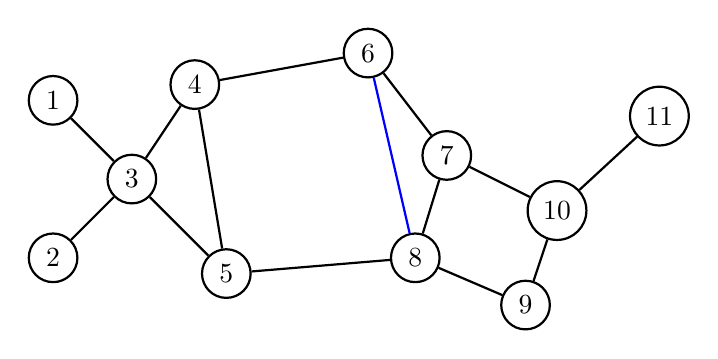
\begin{tikzpicture}
      \begin{scope}[every node/.style={circle,thick,draw}]
        \node (1) at (0,2) {1};
        \node (2) at (0,0) {2};
        \node (3) at (1,1) {3};
        \node (4) at (1.8,2.2) {4};
        \node (5) at (2.2,-0.2) {5};
        \node (6) at (4,2.6) {6};
        \node (7) at (5,1.3) {7};
        \node (8) at (4.6,0) {8};
        \node (9) at (6,-0.6) {9};
        \node (10) at (6.4,0.6) {10};
        \node (11) at (7.7,1.8) {11};
      \end{scope}
      \begin{scope}[every edge/.style={draw,thick}]
        \path (1) edge (3);
        \path (2) edge (3);
        \path (3) edge (4);
        \path (3) edge (5);
        \path (4) edge (5);
        \path (4) edge (6);
        \path (5) edge (8);
        \path (6) edge (7);
        \path (7) edge (8);
        \path (7) edge (10);
        \path (8) edge (9);
        \path (9) edge (10);
        \path (10) edge (11);
        \path[color=blue] (6) edge (8);
      \end{scope}
    \end{tikzpicture}
  \end{center}
\end{frame}


%===== DeepWalk =====

\begin{frame}{An overview of the talk}
  \begin{enumerate}
    \item What is a graph?
    \item Which machine learning tasks can we do on graphs?
      \begin{enumerate}
        \item Node classification
        \item Graph classification
        \item Link prediction
      \end{enumerate}
    \item<alert@1> A zoo of algorithms
      \begin{enumerate}
        \item<alert@2> Transductive classification: DeepWalk
        \item Inductive classification: Graph convolutions
      \end{enumerate}
    \item PyTorch implementation
    \item Application: Fraud detection
  \end{enumerate}
\end{frame}

\begin{frame}{Transductive classification: DeepWalk}
  \invisible{For every node...}
  \invisible{Go for a random {\color{red}walk}...}
  \begin{center}
    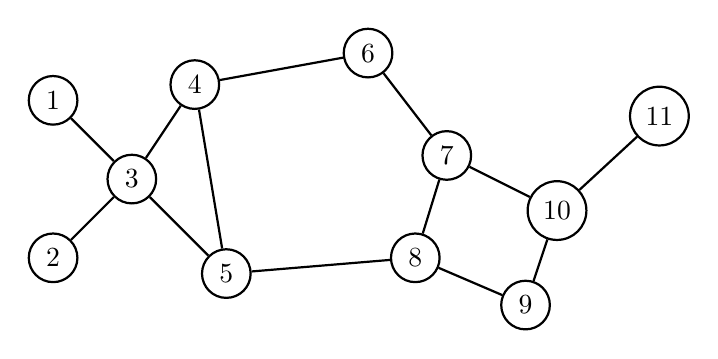
\begin{tikzpicture}
      \begin{scope}[every node/.style={circle,thick,draw}]
        \node (1) at (0,2) {1};
        \node (2) at (0,0) {2};
        \node (3) at (1,1) {3};
        \node (4) at (1.8,2.2) {4};
        \node (5) at (2.2,-0.2) {5};
        \node (6) at (4,2.6) {6};
        \node (7) at (5,1.3) {7};
        \node (8) at (4.6,0) {8};
        \node (9) at (6,-0.6) {9};
        \node (10) at (6.4,0.6) {10};
        \node (11) at (7.7,1.8) {11};
      \end{scope}
      \begin{scope}[every edge/.style={draw,thick}]
        \path (1) edge (3);
        \path (2) edge (3);
        \path (3) edge (4);
        \path (3) edge (5);
        \path (4) edge (5);
        \path (4) edge (6);
        \path (5) edge (8);
        \path (6) edge (7);
        \path (7) edge (8);
        \path (7) edge (10);
        \path (8) edge (9);
        \path (9) edge (10);
        \path (10) edge (11);
      \end{scope}
    \end{tikzpicture}
  \end{center}
\end{frame}

\begin{frame}{Transductive classification: DeepWalk}
  For every {\color{blue}node}...
  \invisible{Go for a random {\color{red}walk}...}
  \begin{center}
    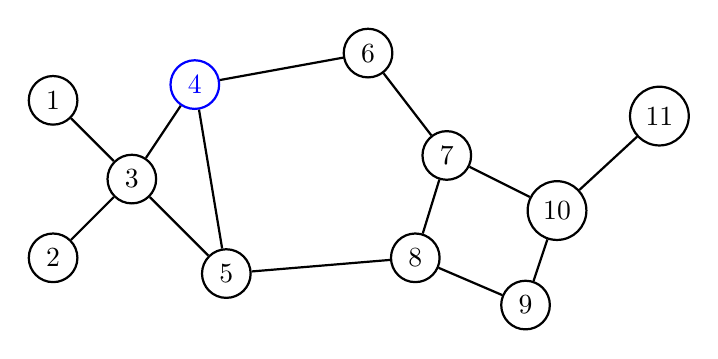
\begin{tikzpicture}
      \begin{scope}[every node/.style={circle,thick,draw}]
        \node (1) at (0,2) {1};
        \node (2) at (0,0) {2};
        \node (3) at (1,1) {3};
        \node[color=blue] (4) at (1.8,2.2) {4};
        \node (5) at (2.2,-0.2) {5};
        \node (6) at (4,2.6) {6};
        \node (7) at (5,1.3) {7};
        \node (8) at (4.6,0) {8};
        \node (9) at (6,-0.6) {9};
        \node (10) at (6.4,0.6) {10};
        \node (11) at (7.7,1.8) {11};
      \end{scope}
      \begin{scope}[every edge/.style={draw,thick}]
        \path (1) edge (3);
        \path (2) edge (3);
        \path (3) edge (4);
        \path (3) edge (5);
        \path (4) edge (5);
        \path (4) edge (6);
        \path (5) edge (8);
        \path (6) edge (7);
        \path (7) edge (8);
        \path (7) edge (10);
        \path (8) edge (9);
        \path (9) edge (10);
        \path (10) edge (11);
      \end{scope}
    \end{tikzpicture}
  \end{center}
\end{frame}

\begin{frame}{Transductive classification: DeepWalk}
  Go for a random {\color{red}walk}...
  \invisible{For every node...}
  \begin{center}
    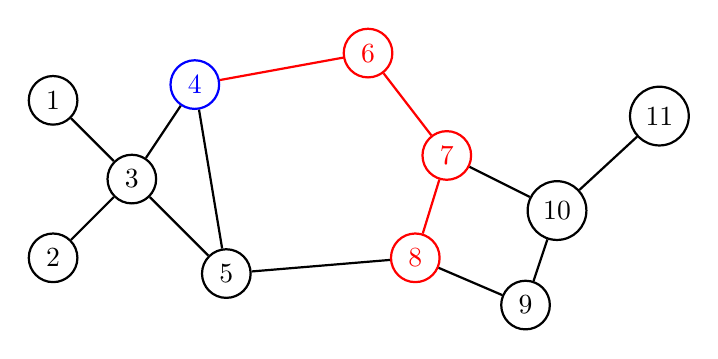
\begin{tikzpicture}
      \begin{scope}[every node/.style={circle,thick,draw}]
        \node (1) at (0,2) {1};
        \node (2) at (0,0) {2};
        \node (3) at (1,1) {3};
        \node[color=blue] (4) at (1.8,2.2) {4};
        \node (5) at (2.2,-0.2) {5};
        \node[color=red] (6) at (4,2.6) {6};
        \node[color=red] (7) at (5,1.3) {7};
        \node[color=red] (8) at (4.6,0) {8};
        \node (9) at (6,-0.6) {9};
        \node (10) at (6.4,0.6) {10};
        \node (11) at (7.7,1.8) {11};
      \end{scope}
      \begin{scope}[every edge/.style={draw,thick}]
        \path (1) edge (3);
        \path (2) edge (3);
        \path (3) edge (4);
        \path (3) edge (5);
        \path (4) edge (5);
        \path[color=red] (4) edge (6);
        \path (5) edge (8);
        \path[color=red] (6) edge (7);
        \path[color=red] (7) edge (8);
        \path (7) edge (10);
        \path (8) edge (9);
        \path (9) edge (10);
        \path (10) edge (11);
      \end{scope}
    \end{tikzpicture}
  \end{center}
\end{frame}

\begin{frame}{Transductive classification: DeepWalk}
  And teach a model to predict the node's neighbours:
  \begin{align*}
    \texttt{model}({\color{blue}4}) \in 
    \{{\color{red}6}, {\color{red}7}, {\color{red}8}\}
  \end{align*}

  \begin{center}
    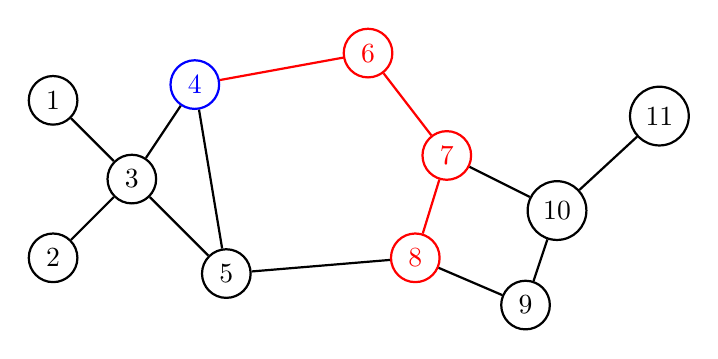
\begin{tikzpicture}
      \begin{scope}[every node/.style={circle,thick,draw}]
        \node (1) at (0,2) {1};
        \node (2) at (0,0) {2};
        \node (3) at (1,1) {3};
        \node[color=blue] (4) at (1.8,2.2) {4};
        \node (5) at (2.2,-0.2) {5};
        \node[color=red] (6) at (4,2.6) {6};
        \node[color=red] (7) at (5,1.3) {7};
        \node[color=red] (8) at (4.6,0) {8};
        \node (9) at (6,-0.6) {9};
        \node (10) at (6.4,0.6) {10};
        \node (11) at (7.7,1.8) {11};
      \end{scope}
      \begin{scope}[every edge/.style={draw,thick}]
        \path (1) edge (3);
        \path (2) edge (3);
        \path (3) edge (4);
        \path (3) edge (5);
        \path (4) edge (5);
        \path[color=red] (4) edge (6);
        \path (5) edge (8);
        \path[color=red] (6) edge (7);
        \path[color=red] (7) edge (8);
        \path (7) edge (10);
        \path (8) edge (9);
        \path (9) edge (10);
        \path (10) edge (11);
      \end{scope}
    \end{tikzpicture}
  \end{center}
\end{frame}

\begin{frame}{Transductive classification: DeepWalk}
  This is done by assigning a learnable vector 
  ${\color{blue}\vec v_i}\in\mathbb R^d$ 
  to every node $i$

  \invisible{asd}

  \invisible{asd}

  \begin{center}
    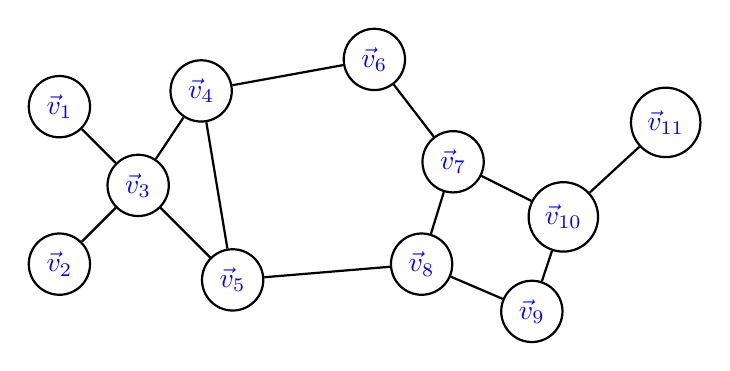
\begin{tikzpicture}
      \begin{scope}[every node/.style={circle,thick,draw}]
        \node (1) at (0,2) {\color{blue}$\vec v_1$};
        \node (2) at (0,0) {\color{blue}$\vec v_2$};
        \node (3) at (1,1) {\color{blue}$\vec v_3$};
        \node (4) at (1.8,2.2) {\color{blue}$\vec v_4$};
        \node (5) at (2.2,-0.2) {\color{blue}$\vec v_5$};
        \node (6) at (4,2.6) {\color{blue}$\vec v_6$};
        \node (7) at (5,1.3) {\color{blue}$\vec v_7$};
        \node (8) at (4.6,0) {\color{blue}$\vec v_8$};
        \node (9) at (6,-0.6) {\color{blue}$\vec v_9$};
        \node (10) at (6.4,0.6) {\color{blue}$\vec v_{10}$};
        \node (11) at (7.7,1.8) {\color{blue}$\vec v_{11}$};
      \end{scope}
      \begin{scope}[every edge/.style={draw,thick}]
        \path (1) edge (3);
        \path (2) edge (3);
        \path (3) edge (4);
        \path (3) edge (5);
        \path (4) edge (5);
        \path (4) edge (6);
        \path (5) edge (8);
        \path (6) edge (7);
        \path (7) edge (8);
        \path (7) edge (10);
        \path (8) edge (9);
        \path (9) edge (10);
        \path (10) edge (11);
      \end{scope}
    \end{tikzpicture}
  \end{center}
\end{frame}

\begin{frame}{Transductive classification: DeepWalk}
  And training a neural network to predict node indices on the
  random walk:
  \begin{align*}
    \texttt{net}({\color{blue}\vec v_4}) = 
      (0, 0, 0, 0, 0, {\color{red}\tfrac{1}{3}}, {\color{red}\tfrac{1}{3}}, 
       {\color{red}\tfrac{1}{3}}, 0, 0, 0)
  \end{align*}

  \begin{center}
    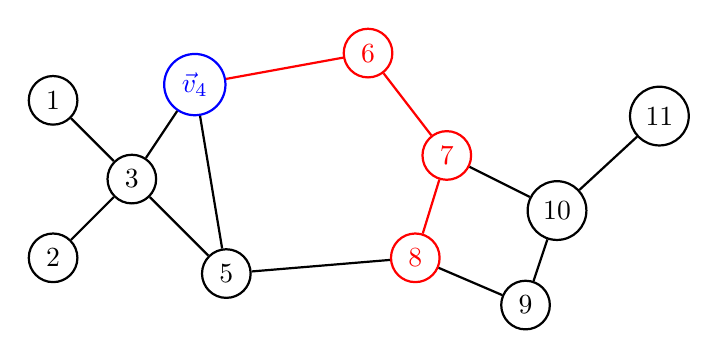
\begin{tikzpicture}
      \begin{scope}[every node/.style={circle,thick,draw}]
        \node (1) at (0,2) {1};
        \node (2) at (0,0) {2};
        \node (3) at (1,1) {3};
        \node[color=blue] (4) at (1.8,2.2) {$\vec v_4$};
        \node (5) at (2.2,-0.2) {5};
        \node[color=red] (6) at (4,2.6) {6};
        \node[color=red] (7) at (5,1.3) {7};
        \node[color=red] (8) at (4.6,0) {8};
        \node (9) at (6,-0.6) {9};
        \node (10) at (6.4,0.6) {10};
        \node (11) at (7.7,1.8) {11};
      \end{scope}
      \begin{scope}[every edge/.style={draw,thick}]
        \path (1) edge (3);
        \path (2) edge (3);
        \path (3) edge (4);
        \path (3) edge (5);
        \path (4) edge (5);
        \path[color=red] (4) edge (6);
        \path (5) edge (8);
        \path[color=red] (6) edge (7);
        \path[color=red] (7) edge (8);
        \path (7) edge (10);
        \path (8) edge (9);
        \path (9) edge (10);
        \path (10) edge (11);
      \end{scope}
    \end{tikzpicture}
  \end{center}
\end{frame}

\begin{frame}{Transductive classification: DeepWalk}
  From these embeddings we can then train any classification model (say,
  logistic regression) to get our node labels:
  \begin{align*}
    \texttt{classificationModel}(\vec v_4) \sim {\color{red}0}\\
    \texttt{classificationModel}(\vec v_7) \sim {\color{blue}1}
  \end{align*}

  \begin{center}
    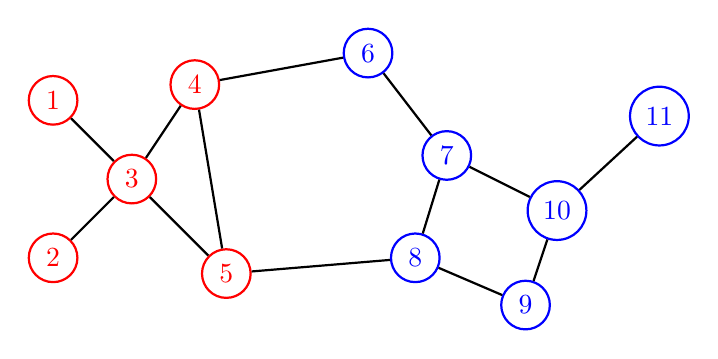
\begin{tikzpicture}
      \begin{scope}[every node/.style={circle,thick,draw}]
        \node[color=red] (1) at (0,2) {1};
        \node[color=red] (2) at (0,0) {2};
        \node[color=red] (3) at (1,1) {3};
        \node[color=red] (4) at (1.8,2.2) {4};
        \node[color=red] (5) at (2.2,-0.2) {5};
        \node[color=blue] (6) at (4,2.6) {6};
        \node[color=blue] (7) at (5,1.3) {7};
        \node[color=blue] (8) at (4.6,0) {8};
        \node[color=blue] (9) at (6,-0.6) {9};
        \node[color=blue] (10) at (6.4,0.6) {10};
        \node[color=blue] (11) at (7.7,1.8) {11};
      \end{scope}
      \begin{scope}[every edge/.style={draw,thick}]
        \path (1) edge (3);
        \path (2) edge (3);
        \path (3) edge (4);
        \path (3) edge (5);
        \path (4) edge (5);
        \path (4) edge (6);
        \path (5) edge (8);
        \path (6) edge (7);
        \path (7) edge (8);
        \path (7) edge (10);
        \path (8) edge (9);
        \path (9) edge (10);
        \path (10) edge (11);
      \end{scope}
    \end{tikzpicture}
  \end{center}
\end{frame}

\begin{frame}{Transductive classification: DeepWalk}
  This algorithm is \alert<1>{transductive}, meaning that we learn a static
  embedding (and thus, classification) for every node.

  If a new node appears, we thus have to train all the embeddings from 
  scratch.

  \pause Note also that this is, by construction, a \alert<2>{proximity
  classification}: nearby nodes will get classified similarly.
\end{frame}

%===== Graph convolutions =====

\begin{frame}{An overview of the talk}
  \begin{enumerate}
    \item What is a graph?
    \item Which machine learning tasks can we do on graphs?
      \begin{enumerate}
        \item Node classification
        \item Graph classification
        \item Link prediction
      \end{enumerate}
    \item A zoo of algorithms
      \begin{enumerate}
        \item Transductive classification: DeepWalk
        \item<alert@1> Inductive classification: Graph convolutions
      \end{enumerate}
    \item PyTorch implementation
    \item Application: Fraud detection
  \end{enumerate}
\end{frame}

\begin{frame}{Inductive classification: Graph convolutions}
  Let's start with a quick recap of what convolutional neural networks 
  are doing.
\end{frame}

\begin{frame}{Inductive classification: Graph convolutions}
  \begin{center}
    \begin{tikzpicture}
      \node (otter) at (0,0) {\includegraphics[scale=0.6]{gfx/otter.jpeg}};
  \end{tikzpicture}
  \end{center}
\end{frame}

\begin{frame}{Inductive classification: Graph convolutions}
  \begin{center}
    \begin{tikzpicture}
      \node (otter) at (0,0) {\includegraphics[scale=0.6]{gfx/otter.jpeg}};
      \draw[draw,thick,color=red] (-5,1.8) rectangle (-4,2.8);
  \end{tikzpicture}
  \end{center}
\end{frame}

\begin{frame}{Inductive classification: Graph convolutions}
  \begin{center}
    \begin{tikzpicture}
      \node (otter) at (0,0) {\includegraphics[scale=0.6]{gfx/otter.jpeg}};
      \draw[draw,thick,color=red] (-4,1.8) rectangle (-3,2.8);
  \end{tikzpicture}
  \end{center}
\end{frame}

\begin{frame}{Inductive classification: Graph convolutions}
  \begin{center}
    \begin{tikzpicture}
      \node (otter) at (0,0) {\includegraphics[scale=0.6]{gfx/otter.jpeg}};
      \draw[draw,thick,color=red] (-3,1.8) rectangle (-2,2.8);
  \end{tikzpicture}
  \end{center}
\end{frame}

\begin{frame}{Inductive classification: Graph convolutions}
  \begin{center}
    \begin{tikzpicture}
      \node (otter) at (0,0) {\includegraphics[scale=0.6]{gfx/otter.jpeg}};
      \draw[draw,thick,color=red] (-2,1.8) rectangle (-1,2.8);
  \end{tikzpicture}
  \end{center}
\end{frame}

\begin{frame}{Inductive classification: Graph convolutions}
  \begin{center}
    \begin{tikzpicture}
      \node (otter) at (0,0) {\includegraphics[scale=0.6]{gfx/otter.jpeg}};
      \draw[draw,thick,color=red] (-1,1.8) rectangle (0,2.8);
  \end{tikzpicture}
  \end{center}
\end{frame}

\begin{frame}{Inductive classification: Graph convolutions}
  \begin{center}
    \begin{tikzpicture}
      \node (otter) at (0,0) {\includegraphics[scale=0.6]{gfx/otter.jpeg}};
      \draw[draw,thick,color=red] (0,1.8) rectangle (1,2.8);
  \end{tikzpicture}
  \end{center}
\end{frame}

\begin{frame}{Inductive classification: Graph convolutions}
  \begin{center}
    \begin{tikzpicture}
      \node (otter) at (0,0) {\includegraphics[scale=0.6]{gfx/otter.jpeg}};
      \draw[draw,thick,color=red] (1,1.8) rectangle (2,2.8);
  \end{tikzpicture}
  \end{center}
\end{frame}

\begin{frame}{Inductive classification: Graph convolutions}
  \begin{center}
    \begin{tikzpicture}
      \node (otter) at (0,0) {\includegraphics[scale=0.6]{gfx/otter.jpeg}};
      \draw[draw,thick,color=red] (2,1.8) rectangle (3,2.8);
  \end{tikzpicture}
  \end{center}
\end{frame}

\begin{frame}{Inductive classification: Graph convolutions}
  \begin{center}
    \begin{tikzpicture}
      \node (otter) at (0,0) {\includegraphics[scale=0.6]{gfx/otter.jpeg}};
      \draw[draw,thick,color=red] (3,1.8) rectangle (4,2.8);
  \end{tikzpicture}
  \end{center}
\end{frame}

\begin{frame}{Inductive classification: Graph convolutions}
  \begin{center}
    \begin{tikzpicture}
      \node (otter) at (0,0) {\includegraphics[scale=0.6]{gfx/otter.jpeg}};
      \draw[draw,thick,color=red] (4,1.8) rectangle (5,2.8);
  \end{tikzpicture}
  \end{center}
\end{frame}

\begin{frame}{Inductive classification: Graph convolutions}
  \begin{center}
    \begin{tikzpicture}
      \node (otter) at (0,0) {\includegraphics[scale=0.6]{gfx/otter.jpeg}};
      \draw[draw,thick,color=red] (-5,0.8) rectangle (-4,1.8);
  \end{tikzpicture}
  \end{center}
\end{frame}

\begin{frame}{Inductive classification: Graph convolutions}
  \begin{center}
    \begin{tikzpicture}
      \node (otter) at (0,0) {\includegraphics[scale=0.6]{gfx/otter.jpeg}};
      \draw[draw,thick,color=red] (-4,0.8) rectangle (-3,1.8);
  \end{tikzpicture}
  \end{center}
\end{frame}

\begin{frame}{Inductive classification: Graph convolutions}
  \begin{center}
    \begin{tikzpicture}
      \node (otter) at (0,0) {\includegraphics[scale=0.6]{gfx/otter.jpeg}};
      \draw[draw,thick,color=red] (-3,0.8) rectangle (-2,1.8);
  \end{tikzpicture}
  \end{center}
\end{frame}

\begin{frame}{Inductive classification: Graph convolutions}
  \begin{center}
    \includegraphics[scale=0.45]{gfx/cnn.png}
    {\tiny [\url{www.mdpi.com/entropy/entropy-19-00242/article_deploy/html/images/entropy-19-00242-g001.png}]}
  \end{center}
\end{frame}

\begin{frame}{Inductive classification: Graph convolutions}
  Let's view the cute otter with our graph hat on.
\end{frame}

\begin{frame}{Inductive classification: Graph convolutions}
  \begin{center}
    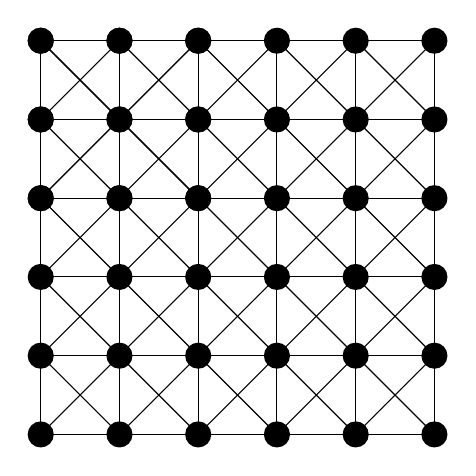
\begin{tikzpicture}

      \begin{scope}[every edge/.style={draw,thick}]
        \foreach \x in {0,...,4}
          \foreach \y in {0,...,4}{
            \draw (\x,\y) -- (\x+1,\y+1);
            \draw (\x,\y) -- (\x+1,\y);
            \draw (\x,\y) -- (\x,\y+1);
            \draw (\x+1,\y) -- (\x,\y+1);
        }
        \foreach \z in {0,...,4}{
          \draw (5,\z) -- (5,\z+1);
          \draw (\z,5) -- (\z+1,5);
        }

        \draw (1,4) -- (0,5);
        \draw (1,4) -- (1,5);
        \draw (1,4) -- (2,5);
        \draw (1,4) -- (0,4);
        \draw (1,4) -- (2,4);
        \draw (1,4) -- (0,3);
        \draw (1,4) -- (1,3);
        \draw (1,4) -- (2,3);
      \end{scope}

      \begin{scope}[every node/.style={circle,thick,fill}]
        \foreach \x in {0,...,5}
          \foreach \y in {0,...,5}
          \node at (\x,\y) {};

        \node at (0,5) {};
        \node at (1,5) {};
        \node at (2,5) {};
        \node at (0,4) {};
        \node at (1,4) {};
        \node at (2,4) {};
        \node at (0,3) {};
        \node at (1,3) {};
        \node at (2,3) {};
      \end{scope}

    \end{tikzpicture}
  \end{center}
\end{frame}

\begin{frame}{Inductive classification: Graph convolutions}
  \begin{center}
    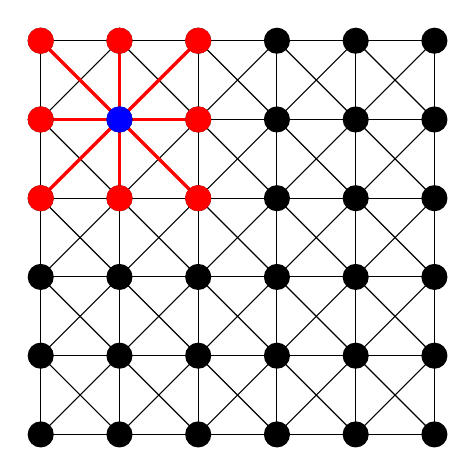
\begin{tikzpicture}

      \begin{scope}[every edge/.style={draw,thick}]
        \foreach \x in {0,...,4}
          \foreach \y in {0,...,4}{
            \draw (\x,\y) -- (\x+1,\y+1);
            \draw (\x,\y) -- (\x+1,\y);
            \draw (\x,\y) -- (\x,\y+1);
            \draw (\x+1,\y) -- (\x,\y+1);
        }
        \foreach \z in {0,...,4}{
          \draw (5,\z) -- (5,\z+1);
          \draw (\z,5) -- (\z+1,5);
        }

        \draw[color=red, very thick] (1,4) -- (0,5);
        \draw[color=red, very thick] (1,4) -- (1,5);
        \draw[color=red, very thick] (1,4) -- (2,5);
        \draw[color=red, very thick] (1,4) -- (0,4);
        \draw[color=red, very thick] (1,4) -- (2,4);
        \draw[color=red, very thick] (1,4) -- (0,3);
        \draw[color=red, very thick] (1,4) -- (1,3);
        \draw[color=red, very thick] (1,4) -- (2,3);
      \end{scope}

      \begin{scope}[every node/.style={circle,thick,fill}]
        \foreach \x in {0,...,5}
          \foreach \y in {0,...,5}
          \node at (\x,\y) {};

        \node[color=red] at (0,5) {};
        \node[color=red] at (1,5) {};
        \node[color=red] at (2,5) {};
        \node[color=red] at (0,4) {};
        \node[color=blue] at (1,4) {};
        \node[color=red] at (2,4) {};
        \node[color=red] at (0,3) {};
        \node[color=red] at (1,3) {};
        \node[color=red] at (2,3) {};
      \end{scope}

    \end{tikzpicture}
  \end{center}
\end{frame}

\begin{frame}{Inductive classification: Graph convolutions}
  \begin{center}
    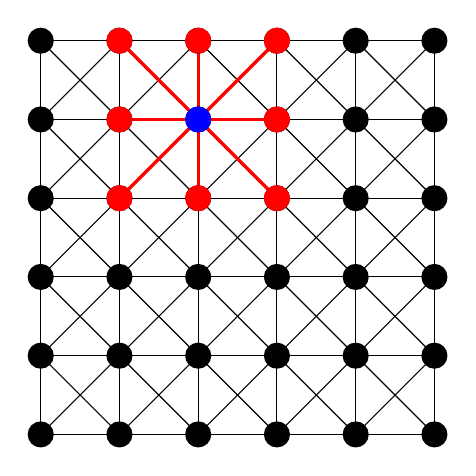
\begin{tikzpicture}

      \begin{scope}[every edge/.style={draw,thick}]
        \foreach \x in {0,...,4}
          \foreach \y in {0,...,4}{
            \draw (\x,\y) -- (\x+1,\y+1);
            \draw (\x,\y) -- (\x+1,\y);
            \draw (\x,\y) -- (\x,\y+1);
            \draw (\x+1,\y) -- (\x,\y+1);
        }
        \foreach \z in {0,...,4}{
          \draw (5,\z) -- (5,\z+1);
          \draw (\z,5) -- (\z+1,5);
        }

        \draw[color=red, very thick] (2,4) -- (1,5);
        \draw[color=red, very thick] (2,4) -- (2,5);
        \draw[color=red, very thick] (2,4) -- (3,5);
        \draw[color=red, very thick] (2,4) -- (1,4);
        \draw[color=red, very thick] (2,4) -- (3,4);
        \draw[color=red, very thick] (2,4) -- (1,3);
        \draw[color=red, very thick] (2,4) -- (2,3);
        \draw[color=red, very thick] (2,4) -- (3,3);
      \end{scope}

      \begin{scope}[every node/.style={circle,thick,fill}]
        \foreach \x in {0,...,5}
          \foreach \y in {0,...,5}
          \node at (\x,\y) {};

        \node[color=red] at (1,5) {};
        \node[color=red] at (2,5) {};
        \node[color=red] at (3,5) {};
        \node[color=red] at (1,4) {};
        \node[color=blue] at (2,4) {};
        \node[color=red] at (3,4) {};
        \node[color=red] at (1,3) {};
        \node[color=red] at (2,3) {};
        \node[color=red] at (3,3) {};
      \end{scope}

    \end{tikzpicture}
  \end{center}
\end{frame}

\begin{frame}{Inductive classification: Graph convolutions}
  \begin{center}
    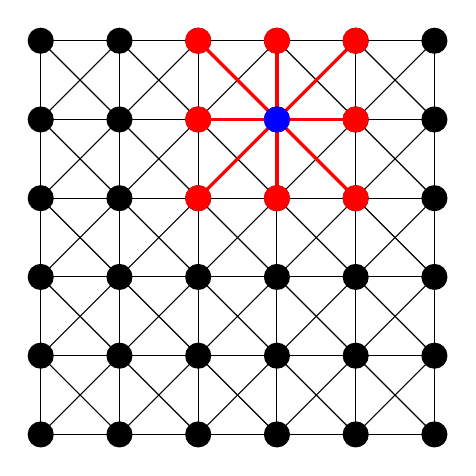
\begin{tikzpicture}

      \begin{scope}[every edge/.style={draw,thick}]
        \foreach \x in {0,...,4}
          \foreach \y in {0,...,4}{
            \draw (\x,\y) -- (\x+1,\y+1);
            \draw (\x,\y) -- (\x+1,\y);
            \draw (\x,\y) -- (\x,\y+1);
            \draw (\x+1,\y) -- (\x,\y+1);
        }
        \foreach \z in {0,...,4}{
          \draw (5,\z) -- (5,\z+1);
          \draw (\z,5) -- (\z+1,5);
        }

        \draw[color=red, very thick] (3,4) -- (2,5);
        \draw[color=red, very thick] (3,4) -- (3,5);
        \draw[color=red, very thick] (3,4) -- (4,5);
        \draw[color=red, very thick] (3,4) -- (2,4);
        \draw[color=red, very thick] (3,4) -- (4,4);
        \draw[color=red, very thick] (3,4) -- (2,3);
        \draw[color=red, very thick] (3,4) -- (3,3);
        \draw[color=red, very thick] (3,4) -- (4,3);
      \end{scope}

      \begin{scope}[every node/.style={circle,thick,fill}]
        \foreach \x in {0,...,5}
          \foreach \y in {0,...,5}
          \node at (\x,\y) {};

        \node[color=red] at (2,5) {};
        \node[color=red] at (3,5) {};
        \node[color=red] at (4,5) {};
        \node[color=red] at (2,4) {};
        \node[color=blue] at (3,4) {};
        \node[color=red] at (4,4) {};
        \node[color=red] at (2,3) {};
        \node[color=red] at (3,3) {};
        \node[color=red] at (4,3) {};
      \end{scope}

    \end{tikzpicture}
  \end{center}
\end{frame}

\begin{frame}{Inductive classification: Graph convolutions}
  \begin{center}
    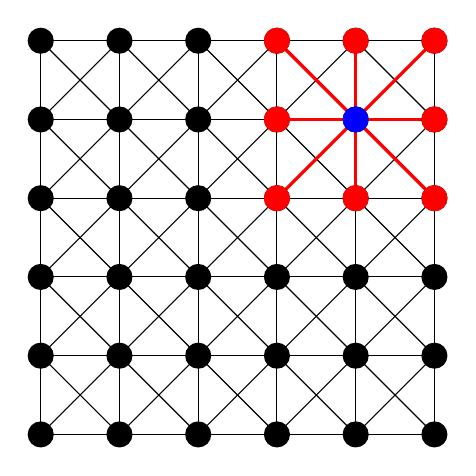
\begin{tikzpicture}

      \begin{scope}[every edge/.style={draw,thick}]
        \foreach \x in {0,...,4}
          \foreach \y in {0,...,4}{
            \draw (\x,\y) -- (\x+1,\y+1);
            \draw (\x,\y) -- (\x+1,\y);
            \draw (\x,\y) -- (\x,\y+1);
            \draw (\x+1,\y) -- (\x,\y+1);
        }
        \foreach \z in {0,...,4}{
          \draw (5,\z) -- (5,\z+1);
          \draw (\z,5) -- (\z+1,5);
        }

        \draw[color=red, very thick] (4,4) -- (3,5);
        \draw[color=red, very thick] (4,4) -- (4,5);
        \draw[color=red, very thick] (4,4) -- (5,5);
        \draw[color=red, very thick] (4,4) -- (3,4);
        \draw[color=red, very thick] (4,4) -- (5,4);
        \draw[color=red, very thick] (4,4) -- (3,3);
        \draw[color=red, very thick] (4,4) -- (4,3);
        \draw[color=red, very thick] (4,4) -- (5,3);
      \end{scope}

      \begin{scope}[every node/.style={circle,thick,fill}]
        \foreach \x in {0,...,5}
          \foreach \y in {0,...,5}
          \node at (\x,\y) {};

        \node[color=red] at (3,5) {};
        \node[color=red] at (4,5) {};
        \node[color=red] at (5,5) {};
        \node[color=red] at (3,4) {};
        \node[color=blue] at (4,4) {};
        \node[color=red] at (5,4) {};
        \node[color=red] at (3,3) {};
        \node[color=red] at (4,3) {};
        \node[color=red] at (5,3) {};
      \end{scope}

    \end{tikzpicture}
  \end{center}
\end{frame}

\begin{frame}{Inductive classification: Graph convolutions}
  Note that every node has the \alert<1>{same number of neighbours} \pause 
  (if we included padding).

  \pause This makes it possible to learn a $3\times 3$ matrix (the
  \alert<3>{kernel}), which we can convolve over:
  \begin{align*}
    (\texttt{pixels}\star\texttt{kernel})_{m,n} :=
    \sum_{i=-1}^1\sum_{j=-1}^1
    \texttt{kernel}_{i,j}\texttt{pixels}_{m\alert<4>{-i},n\alert<4>{-j}}
  \end{align*}

  \pause Crucially, for this to work, we are able \alert<4>{shift} in the
  $x$- and/or $y$-direction. 

  \pause We lose this feature for general graphs, so what do we do?
\end{frame}

\begin{frame}{Inductive classification: Graph convolutions}
  \centering\Large MATHS
\end{frame}

\begin{frame}{Inductive classification: Graph convolutions}
  \begin{block}{The Convolution Theorem}
    Convolutions between two functions $f,g\colon\mathbb R^n\to\mathbb R$ 
    are equivalent to element-wise multiplication in the Fourier domain:
    \begin{align*}
      \texttt{fourier}(f\star g) = 
      \texttt{fourier}(f)\cdot\texttt{fourier}(g)
    \end{align*}
  \end{block}

  \pause One can define a version of the Fourier transform applied to 
  functions on nodes of a graph, call it $\texttt{graphFourier}$, and then
  define the graph convolution as
  \begin{align*}
    f\star g := 
    \texttt{graphFourier}^{-1}(
    \texttt{graphFourier}(f)\cdot\texttt{graphFourier}(g))
  \end{align*}

  \pause This is called a \alert<3>{spectral graph convolution}.
\end{frame}

\begin{frame}{Inductive classification: Graph convolutions}
  The problem is that spectral graph convolutions are 
  \alert<1>{computationally expensive} ($\mathcal O(\texttt{numNodes}^2)$).

  \pause However, Hammond et al. (2011) from EPFL in Lausanne came up 
  with an approximation of the graph Fourier transform.

  \pause Kipf and Welling (2017) from the University of Amsterdam used
  this to construct an approximation to the spectral graph convolution 
  which is $\mathcal O(\texttt{numEdges})$.

  \pause This approximation is also quite simple. Let's have a look.
\end{frame}

\begin{frame}{Inductive classification: Graph convolutions}

  Say we want to compute the convolution at node $\color{blue}4$.

  \begin{center}
    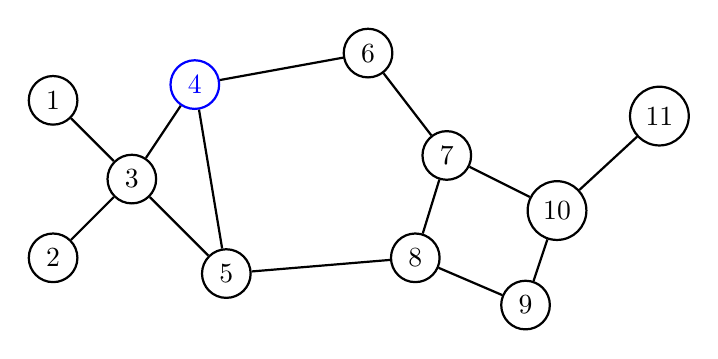
\begin{tikzpicture}
      \begin{scope}[every node/.style={circle,thick,draw}]
        \node (1) at (0,2) {1};
        \node (2) at (0,0) {2};
        \node (3) at (1,1) {3};
        \node[color=blue] (4) at (1.8,2.2) {4};
        \node (5) at (2.2,-0.2) {5};
        \node (6) at (4,2.6) {6};
        \node (7) at (5,1.3) {7};
        \node (8) at (4.6,0) {8};
        \node (9) at (6,-0.6) {9};
        \node (10) at (6.4,0.6) {10};
        \node (11) at (7.7,1.8) {11};
      \end{scope}
      \begin{scope}[every edge/.style={draw,thick}]
        \path (1) edge (3);
        \path (2) edge (3);
        \path (3) edge (4);
        \path (3) edge (5);
        \path (4) edge (5);
        \path (4) edge (6);
        \path (5) edge (8);
        \path (6) edge (7);
        \path (7) edge (8);
        \path (7) edge (10);
        \path (8) edge (9);
        \path (9) edge (10);
        \path (10) edge (11);
      \end{scope}
    \end{tikzpicture}
  \end{center}
\end{frame}

\begin{frame}{Inductive classification: Graph convolutions}

  For every {\color{red}neighbour} of $\color{blue}4$...

  \begin{center}
    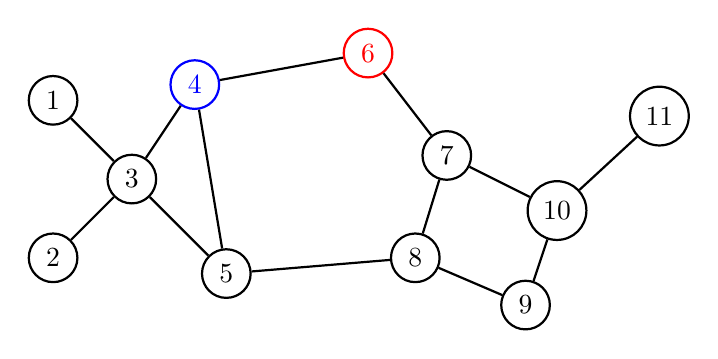
\begin{tikzpicture}
      \begin{scope}[every node/.style={circle,thick,draw}]
        \node (1) at (0,2) {1};
        \node (2) at (0,0) {2};
        \node (3) at (1,1) {3};
        \node[color=blue] (4) at (1.8,2.2) {4};
        \node (5) at (2.2,-0.2) {5};
        \node[color=red] (6) at (4,2.6) {6};
        \node (7) at (5,1.3) {7};
        \node (8) at (4.6,0) {8};
        \node (9) at (6,-0.6) {9};
        \node (10) at (6.4,0.6) {10};
        \node (11) at (7.7,1.8) {11};
      \end{scope}
      \begin{scope}[every edge/.style={draw,thick}]
        \path (1) edge (3);
        \path (2) edge (3);
        \path (3) edge (4);
        \path (3) edge (5);
        \path (4) edge (5);
        \path (4) edge (6);
        \path (5) edge (8);
        \path (6) edge (7);
        \path (7) edge (8);
        \path (7) edge (10);
        \path (8) edge (9);
        \path (9) edge (10);
        \path (10) edge (11);
      \end{scope}
    \end{tikzpicture}
  \end{center}
\end{frame}

\begin{frame}{Inductive classification: Graph convolutions}

  We take its feature vector and normalise it by both {\color{red}it}'s 
  and $\color{blue}4$'s degrees...
  \begin{align*}
    h_6 := \frac{\vec v_6}{\sqrt{\texttt{degree}(4)\texttt{degree}(6)}} 
    = \frac{\vec v_6}{\sqrt{3\cdot 2}}
  \end{align*}

  \begin{center}
    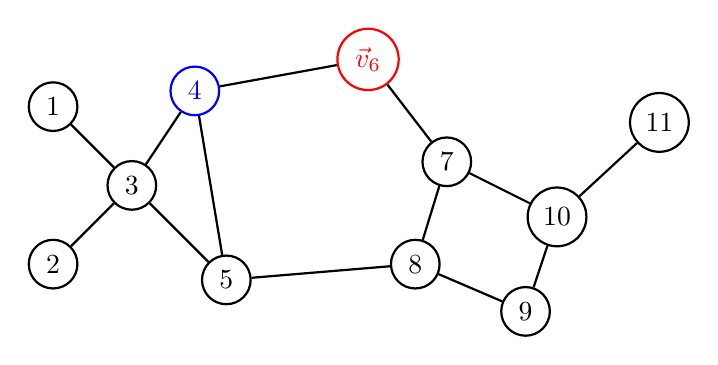
\begin{tikzpicture}
      \begin{scope}[every node/.style={circle,thick,draw}]
        \node (1) at (0,2) {1};
        \node (2) at (0,0) {2};
        \node (3) at (1,1) {3};
        \node[color=blue] (4) at (1.8,2.2) {4};
        \node (5) at (2.2,-0.2) {5};
        \node[color=red] (6) at (4,2.6) {$\vec v_6$};
        \node (7) at (5,1.3) {7};
        \node (8) at (4.6,0) {8};
        \node (9) at (6,-0.6) {9};
        \node (10) at (6.4,0.6) {10};
        \node (11) at (7.7,1.8) {11};
      \end{scope}
      \begin{scope}[every edge/.style={draw,thick}]
        \path (1) edge (3);
        \path (2) edge (3);
        \path (3) edge (4);
        \path (3) edge (5);
        \path (4) edge (5);
        \path (4) edge (6);
        \path (5) edge (8);
        \path (6) edge (7);
        \path (7) edge (8);
        \path (7) edge (10);
        \path (8) edge (9);
        \path (9) edge (10);
        \path (10) edge (11);
      \end{scope}
    \end{tikzpicture}
  \end{center}
\end{frame}

\begin{frame}{Inductive classification: Graph convolutions}

  Node $\color{blue}4$'s new value is then the sum of the $h_i$'s, multiplied
  with a learnable weight matrix $W$:
  \begin{align*}
    {\color{blue}\vec v_4} := W({\color{blue}h_4} + {\color{red}h_3} + 
    {\color{red}h_5} + {\color{red}h_6})
  \end{align*}

  \begin{center}
    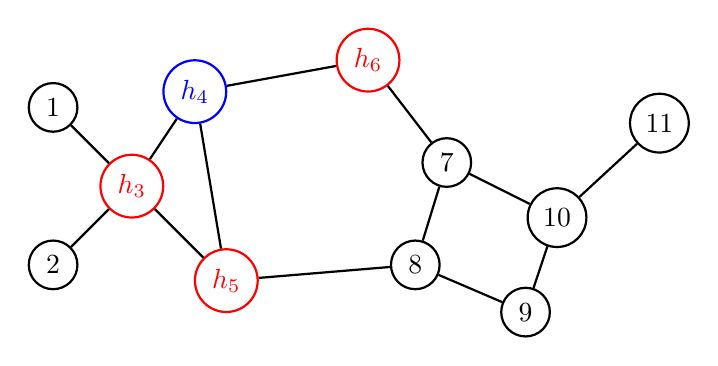
\begin{tikzpicture}
      \begin{scope}[every node/.style={circle,thick,draw}]
        \node (1) at (0,2) {1};
        \node (2) at (0,0) {2};
        \node[color=red] (3) at (1,1) {$h_3$};
        \node[color=blue] (4) at (1.8,2.2) {$h_4$};
        \node[color=red] (5) at (2.2,-0.2) {$h_5$};
        \node[color=red] (6) at (4,2.6) {$h_6$};
        \node (7) at (5,1.3) {7};
        \node (8) at (4.6,0) {8};
        \node (9) at (6,-0.6) {9};
        \node (10) at (6.4,0.6) {10};
        \node (11) at (7.7,1.8) {11};
      \end{scope}
      \begin{scope}[every edge/.style={draw,thick}]
        \path (1) edge (3);
        \path (2) edge (3);
        \path (3) edge (4);
        \path (3) edge (5);
        \path (4) edge (5);
        \path (4) edge (6);
        \path (5) edge (8);
        \path (6) edge (7);
        \path (7) edge (8);
        \path (7) edge (10);
        \path (8) edge (9);
        \path (9) edge (10);
        \path (10) edge (11);
      \end{scope}
    \end{tikzpicture}
  \end{center}
\end{frame}

\begin{frame}{Inductive classification: Graph convolutions}
  This algorithm is \alert<1>{inductive}, meaning that if a new node appears 
  in the graph, then we use the pre-trained model to do inference on it

  \pause As opposed to DeepWalk, the GCNs are inherently 
  \alert<2>{supervised}, but methods exist to train this in an unsupervised 
  way (e.g. the Deep Graph Infomax algorithm from 
  Veli\v ckovi\'c et al., 2018)
\end{frame}

%===== PyTorch implementation =====

\begin{frame}{An overview of the talk}
  \begin{enumerate}
    \item What is a graph?
    \item Which machine learning tasks can we do on graphs?
      \begin{enumerate}
        \item Node classification
        \item Graph classification
        \item Link prediction
      \end{enumerate}
    \item A zoo of algorithms
      \begin{enumerate}
        \item Transductive classification: DeepWalk
        \item Inductive classification: Graph convolutions
      \end{enumerate}
    \item<alert@1> PyTorch implementation
    \item Application: Fraud detection
  \end{enumerate}
\end{frame}

\begin{frame}{PyTorch implementation}
  Deep Graph Library: {\footnotesize\url{https://www.dgl.ai}}

  \pause\scriptsize
  \tt{import torch}\\
  \tt{import torch.nn as nn}\\
  \alert<3>{\tt{import dgl}}\\
  \alert<3>{\tt{import dgl.nn.pytorch as dglnn}}

  \tt{class GCN(nn.Module):}\\
  \qquad\tt{def \_\_init\_\_(self, in\_feats:int, hidden\_size:int,
  num\_classes:int):}\\
  \qquad\qquad\tt{super().\_\_init\_\_()}\\
  \qquad\qquad\tt{self.conv1 = 
  \alert<3>{dglnn.GraphConv(in\_feats, hidden\_size)}}\\
  \qquad\qquad\tt{self.conv2 = 
  \alert<3>{dglnn.GraphConv(hidden\_size, num\_classes)}}

  \qquad\tt{def forward(self, \alert<4>{graph:dgl.DGLGraph}, 
  x:torch.tensor):}\\
  \qquad\qquad\tt{x = self.conv1(\alert<4>{graph}, x)}\\
  \qquad\qquad\tt{x = torch.relu(x)}\\
  \qquad\qquad\tt{x = self.conv2(\alert<4>{graph}, x)}\\
  \qquad\qquad\tt{return x}
\end{frame}

\begin{frame}{PyTorch implementation}
  PyTorch Geometric:
  {\footnotesize\url{https://github.com/rusty1s/pytorch_geometric}}

  \pause\scriptsize
  \tt{import torch}\\
  \tt{import torch.nn as nn}\\
  \alert<3>{\tt{import torch\_geometric as tg}}\\
  \alert<3>{\tt{import torch\_geometric.nn as tgnn}}

  \tt{class GCN(nn.Module):}\\
  \qquad\tt{def \_\_init\_\_(self, in\_feats:int, hidden\_size:int,
  num\_classes:int):}\\
  \qquad\qquad\tt{super().\_\_init\_\_()}\\
  \qquad\qquad\tt{self.conv1 = 
  \alert<3>{tgnn.GCNConv(in\_feats, hidden\_size)}}\\
  \qquad\qquad\tt{self.conv2 = 
  \alert<3>{tgnn.GCNConv(hidden\_size, num\_classes)}}

  \qquad\tt{def forward(self, \alert<4>{data:tg.data.Data}):}\\
  \qquad\qquad\tt{\alert<4>{x, edge\_index = data.x, data.edge\_index}}\\
  \qquad\qquad\tt{x = self.conv1(x, \alert<4>{edge\_index})}\\
  \qquad\qquad\tt{x = torch.relu(x)}\\
  \qquad\qquad\tt{x = self.conv2(x, \alert<4>{edge\_index})}\\
  \qquad\qquad\tt{return x}
\end{frame}


%===== Application: Fraud detection =====

\begin{frame}{An overview of the talk}
  \begin{enumerate}
    \item What is a graph?
    \item Which machine learning tasks can we do on graphs?
      \begin{enumerate}
        \item Node classification
        \item Graph classification
        \item Link prediction
      \end{enumerate}
    \item A zoo of algorithms
      \begin{enumerate}
        \item Transductive classification: DeepWalk
        \item Inductive classification: Graph convolutions
      \end{enumerate}
    \item PyTorch implementation
    \item<alert@1> Application: Fraud detection
  \end{enumerate}
\end{frame}

\begin{frame}{Application: Fraud detection}
  The \alert<1>{Danish Business Authority} endeavours to create the best 
  conditions for \alert<1>{growth} in Europe, and to make it \alert<1>{easy} 
  and \alert<1>{attractive} to run a business in Denmark.

  \pause All companies in Denmark \alert<2>{have to register} with the 
  authority before they are officially recognised as a company.
\end{frame}

\begin{frame}{Application: Fraud detection}
  The authority has a \alert<1>{machine learning lab}, who works with
  \alert<1>{assisted tax fraud detection}.

  \pause No decisions are taken based on algorithms, however.

  \pause The lab has access to data from other authorities, like data about
  VAT, tax and income.
\end{frame}

\begin{frame}{Application: Fraud detection}
  Most of our data is organised in a \alert<1>{Neo4j graph database}.

  \begin{center}
    \scriptsize
    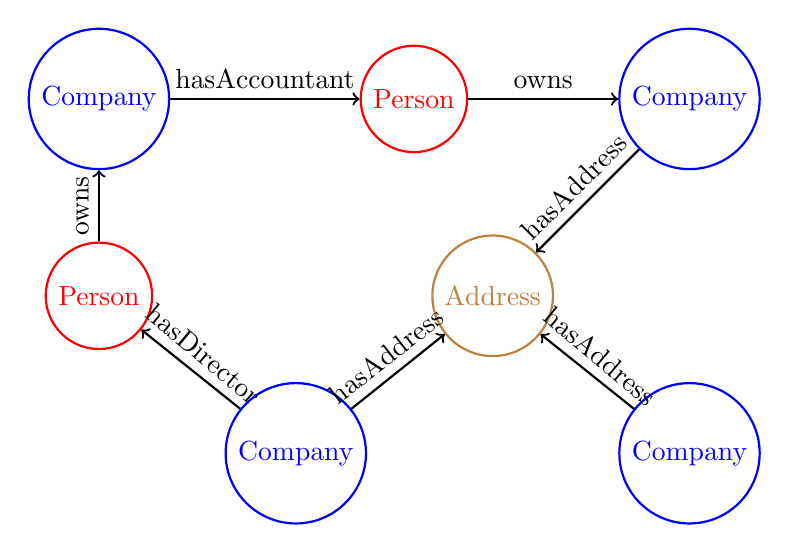
\begin{tikzpicture}
      \begin{scope}[every node/.style={circle,thick,draw}]
        \node[color=blue] (company1) at (0,0) {Company};
        \node[color=red] (owner) at (0,-2.5) {Person};
        \node[color=blue] (company2) at (2.5,-4.5) {Company};
        \node[color=brown] (address) at (5,-2.5) {Address};
        \node[color=blue] (company3) at (7.5,0) {Company};
        \node[color=red] (accountant) at (4,0) {Person};
        \node[color=blue] (company4) at (7.5,-4.5) {Company};
      \end{scope}
      \begin{scope}[every edge/.style={draw,thick,->}]
        \path (owner) edge node[rotate=90, above] {owns} (company1);
        \path (company2) edge node[rotate=-40, above] {hasDirector} (owner);
        \path (company2) edge node[rotate=38, above] {hasAddress} (address);
        \path (company3) edge node[rotate=45, above] {hasAddress} (address);
        \path (company1) edge node[above] {hasAccountant} (accountant);
        \path (accountant) edge node[above] {owns} (company3);
        \path (company4) edge node[rotate=-40, above] {hasAddress} (address);
      \end{scope}
    \end{tikzpicture}
  \end{center}

\end{frame}

\begin{frame}{Application: Fraud detection}
  This database currently have more than 300 million nodes and 500 
  million relations.

  \pause So far we have been using manually curated graph features in our
  machine learning models.

  \pause We are currently in the process of implementing graph neural 
  networks to automate this, and (hopefully!) improve the performance of the
  models as well.
\end{frame}

\begin{frame}{The End}
  \centering\Large Thank you for your attention.
\end{frame}

\end{document}
